\chapter{Self-sovereign Identity}\label{chapter: ssi}

% Topic: Identity is extremely important!
Health care, social security, education, access to financial services — this is just a small list of requirements that are essential for a decent life and are usually taken for granted by people in the Western world. Yet, there are more than 1.1 billion people worldwide who cannot provide identification and thus cannot access the most basic services. Digital identities could make a significant contribution towards solving this problem and giving people the chance to participate in society on a more equal playing field. \cite{world_bank_11_2017}

% Topic: We haven't figured it out yet though...
As already mentioned in chapter \ref{chapter: Introduction}, however, current implementations of such digital identities are insufficient for the problems of our modern times. \cite{soltani_survey_2021} divided these problems into four categories:
\begin{enumerate}
	\item Data Ownership and Governance
	\item Password-Based Authentication
	\item Fragmented Identity Data
	\item Data Breaches and Identity Fraud
\end{enumerate}
The former describes the fact that users have no ownership over their digital identities and thus cannot exercise any control over them. Service providers often take advantage of this and use collected data to create comprehensive profiles of their users and thus sell tailored advertising space on corresponding marketplaces for high figures. The lack of control also means that service providers can temporarily or permanently deny users access to their digital identity at any time. At the beginning of 2021, this led to much discussion as the account of former U.S. President Donald Trump was permanently banned from Twitter. One of the central concerns was whether service providers have too much power over users' liberties \cite{noor_should_2021}. In addition, given the frequent and often repeated use of weak passwords, the heavy reliance on password-based authentication is a security risk that may lead to identity theft. If users want to protect themselves, they need to use different and complex passwords for each of their accounts, which quickly becomes a complicated undertaking without a password manager. A study by the password manager LastPass, for example, found that a business customer manages an average of 191 passwords \cite{steel_lastpass_2017}. While the use of such tools greatly simplifies the management of passwords, they too can pose a major security risk and do not completely protect the user \cite{oesch_that_2020, ormandy_password_2021, toth_you_2021}. Alternatives such as single sign-on, where users authenticate to other service providers using for example their Google account, can solve this problem but lead to even greater dependency and centralization. The third issue involves identity data being spread across a large set of service providers, making it difficult to maintain. As a result, duplicates, errors, and outdated data sets are common. The lack of open standards also complicates interoperability between providers, which could theoretically be used to retrieve, move, or delete personal data. Efforts like the Data Transfer Project founded by Microsoft, Google, Twitter, and Facebook try to simplify the transfer of data between providers, but after more than 3 years show very few actual successes \cite{minor_google_2020, hollington_surprising_2021, lomas_facebooks_2020} and are being criticized for pushing small competitors even further behind \cite[p. 15]{borgogno_data_2018}. \cite[pp. 2-3]{soltani_survey_2021}

One of the biggest problems, however, are data breaches. In June 2021 alone, there were 235 breaches with 1.16 billion stolen records, with a total of 18.9 billion records stolen in 1,785 breaches in the first half of 2021 \cite{risk_based_security_data_2021}. Looking at the past, there have been quite a few major hacks \cite{swinhoe_15_2021}, including: 

\begin{itemize}
    \item Yahoo (2013): 3 billion accounts
    \item Marriott (2018): 500 million customer records
    \item Alibaba (2019): 1.1 billion entries
    \item LinkedIn (2021): 700 million accounts
\end{itemize}

A survey of 413 people by \cite{mayer_now_2021} found that 73\% of participants had been affected by at least one, but an average of 5.3 data breaches. In addition, the majority blamed themselves for the breaches, with only 14\% aware that service providers were responsible.

These are decades-old problems that were already critically discussed by Kim Cameron in 2005. Cameron, who last worked as Chief Architect of Identity at Microsoft from 1999 to 2019, wrote the following on a blog article \cite{cameron_laws_2005}:

\begin{displayquote}
    \textit{“The Internet was built without a way to know who and what you are connecting to. This limits what we can do with it and exposes us to growing dangers. If we do nothing, we will face rapidly proliferating episodes of theft and deception that will cumulatively erode public trust in the Internet.”}
\end{displayquote}

Cameron attributes these problems to the lack of an identity layer on the Internet, which has resulted in many services having to find their own solutions. He calls this a \textit{patchwork of identity one-offs}, which fundamentally still exists today and is difficult to resolve. The reason for this, he says, is a lack of consensus and an unwillingness to give up too much control over identity data. A solution for this is, according to him, an \textit{identity metasystem} that abstracts away deeper complexities similar to hardware drivers or TCP/IP and only loosely couples digital identities to the systems.  Such an open identity layer could only be successful if it fulfilled the seven laws of identity defined by Cameron. These include criteria such as user control, consent, pluralism and minimal disclosure. \cite{cameron_laws_2005}

Over the years, these ideas, among others like \cite{devon_what_2012, idcubedorg_id3_2014, allen_path_2016}, gave rise to the concept of \acf{SSI}. It is intended to eliminate the shortcomings of today's established concepts by placing the users in the center and giving them back complete control over their identity data. A user can decide what, to whom and how much data is shared without being dependent on a central authority. The emergence of blockchain technology and various new standards in recent years gave a new boost to implement \ac{SSI} in reality. [\citealp[pp. 6-7]{struker_grundlagen_2021}; \citealp[pp. 8-9]{tobin_inevitable_2017}]

\ac{SSI} is an entirely new approach to digital identities on the Internet and is seen as a paradigm shift that deeply affects the infrastructure and power distribution of the Internet \cite[p. 3]{preukschat_self-sovereign_2021}. For a more profound look at the topic, this chapter takes a closer look at Self-sovereign Identity. To do so, the concept of identity and the different types of identities will be discussed first. This is followed by a historical look at the different stages of digital identities, taking a closer look at the previous concepts of \ac{SSI}. After a basic foundation has been built, standards that have been established in recent years and are intended to make \ac{SSI} feasible in reality are described. Finally, the \ac{SSI} architecture with its components and roles will be looked at.

% Next: Maybe add a short Intro like i did in chapter 1. --> Definition, Motivation, Problem Definition, Vision

    \section{Identity}

    What defines a human being? One would probably get various answers to this question, such as its name, gender, place of residence, profession, hobbies, religion, charitable activities, party affiliation or even a combination of all these characteristics. \cite[p. 206]{claus_identity_2001} describes in his work that a person's identity is not just a single, fixed construct, but consists of several partial identities. Thus, depending on the context in which a person finds itself, it takes on one of its various partial identities, which represents it as a human being more or less. For example, a partial identity for health care consists of its medical history, while the partial identity towards work contains received certificates. Nevertheless, these different parts of the identity are not necessarily considered separately, as they can also overlap in certain aspects of information. It is important to mention that a person decides which information to share at which time towards which entity. In figure \ref{figure: alice} the concept of partial identities is illustrated exemplarily by a person Alice.
    
    \begin{figure}[ht]
        \centering
        \makebox[\textwidth]{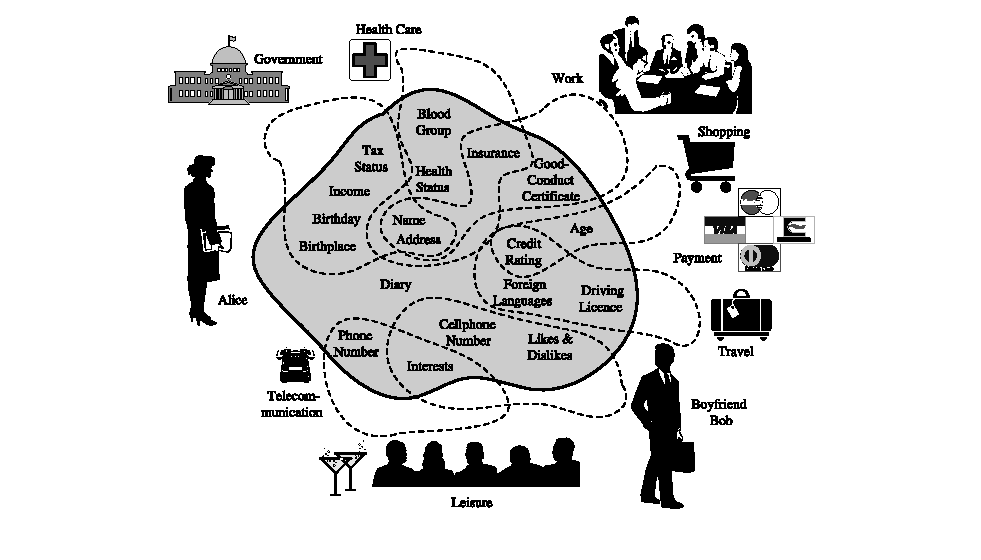
\includegraphics[width=\textwidth]{img/2_alice.eps}}
        \caption{Partial Identities of Alice extracted from \cite{claus_identity_2001}}
        \label{figure: alice}
    \end{figure}

    An important balancing act is to disclose the right amount of data to maintain anonymity, but also to provide the other person with the necessary information. For the purchase of a water, the kiosk vendor should not ask for any personal data, whereas verification of age when buying alcohol is a valid reason for information disclosure. In reality, official documents, such as state identification documents, or sometimes unofficial documents, such as customer cards, are usually used for such proof of identity. Here, users have full control over their documents as they are under their control, and only they can decide self-sovereignly whom and when to show them. Official identification documents are also produced and standardized to ensure the highest possible level of security and interoperability. Other countries can verify such documents without explicitly contacting authorities, simply by looking at the document. Confidence in the validity of the data arises from the fact that the verifying party trusts the authority issuing the document. \cite[p. 6]{struker_grundlagen_2021}

    As a result of the increasing digitalization of various branches of life, many processes are shifting to the digital world. Digital identities, which are similar to analogue identities in terms of their basic idea, are now being used for interacting with digital services. They allow entities, such as people or objects, to authenticate themselves online through certain attributes and thus prove their identity [\citealp[p. 103]{meinel_blockchain_2020}; \citealp{bundesdruckerei_so_2020}]. A more precise definition is given by Cameron \cite{cameron_laws_2005}, who defines digital identity as \textit{“A set of assertions that a digital subject makes about itself or another digital subject”}. In this context, a digital subject is \textit{“A person or thing represented or existing in the digital realm which is being described or dealt with.”} and the attributes mentioned can be represented in the form of claims, which are defined as \textit{“An assertion of the truth of something, typically one which is disputed or doubted”}. The problem is that analogue identities and their documents usually have no or not widely accepted \cite{krempl_e-government-studie_2019, koppenhofer_kabinettsbeschluss_2021} digital representations that could be used as a digital identity. From this emerged the patchwork of identity one-offs described in chapter \ref{chapter: ssi}, resulting in a divergence of digital identities from their original counterparts concerning their characteristics. To better understand this development, the next section describes the different stages of digital identities in more detail. [\citealp[p. 10]{struker_grundlagen_2021}; \citealp[p. 2]{ehrlich_self-sovereign_2021}]
    
	\section{Stages}
	
	As indicated in the last section, Allen's work \cite{allen_path_2016} has had a major influence on what is today considered Self-sovereign Identity and has been cited in over 100 works according to Google Scholar. According to him, digital identities, or online identities, have gone through four major stages since the beginning of the internet. These are examined in more detail below and show which developments led to the emergence of \ac{SSI}.
	
	    \subsection{Centralized Identity}
	    Centralized identities are identities that are issued and verified by a single party or hierarchy. The oldest examples of this are IANA (1988) for the administration of IP addresses, ICANN (1998) for domain names and \acfp{ca}, which play a major role today, particularly in connection with SSL certificates. Especially with the latter, the hierarchical structure of \acp{ca} becomes obvious when one looks at an SSL certificate in the browser. Here, a root authority allows another organization to manage its own hierarchy, while at all times the root authority has full control. This is highly critical for numerous reasons. For example, one entity has complete control over identities and can delete them at any time or even issue false identities. The latter can happen both willingly and unwillingly as a result of a hack. Due to the centralized nature of such authorities, they and thus also the complete hierarchy (chain of trust) are targets of attack, which has been shown in recent years \cite{borchers_diginotar-ssl-gau_2012}. Just like these organizations, due to the lack of an identity layer, all services on the internet developed similar centralized solutions (see chapter \ref{chapter: ssi}. This manifests itself above all in the various accounts that an internet user has to manage for various services. Again, users have little control over their data. \cite{allen_path_2016}
	    
	    In addition, the user has to manage the abundance of login credentials efficiently and securely. However, it is also a challenge for the services, as they have to store a large amount of sensitive data securely and in compliance with data protection laws. Nevertheless, the beneficiaries here are the services, as they can act flexibly and independently of third parties and have full control over the data. \cite[p. 6]{ehrlich_self-sovereign_2021}
	    
	    
	    \subsection{Federated Identity}
	    
	    The second stage of development is represented by the so-called federated identities, which were intended to break down the hierarchies based on a single authority. Here, various commercial organizations developed a model in which control was to be divided between several federated authorities. One of the first projects in this area was Microsoft's Passport in 1999, where Microsoft created a single, federated identity for users that could be used on multiple sites. However, this unification came with the price that Microsoft was now at the center of the federation and could thus exert full control. Other efforts, such as Liberty Alliance Project, founded in 2001, attempted to create an actual federation between multiple companies in which control was distributed among them. The result, however, was a kind of oligarchy in which users still had no control over their data. In the end, the sites remained authorities. \cite{allen_path_2016}
	    
	    Nevertheless, this type of digital identity is advantageous in that users do not have to manage an identity/ account for each service and companies have less administrative effort. The identity provider, e.g., Microsoft, acts as the issuer and owner of the data and is thus the central point of contact if a user wants to log on to another service of the federation. The user therefore has no control over his data and is dependent on the continued existence of the identity provider. Due to the abundance of sensitive data, it is possible for the identity provider to aggregate information from various areas in order to create user profiles, which in itself can lead to various problems. \cite[pp. 6 - 7]{ehrlich_self-sovereign_2021}
	    
	    \subsection{User-Centric Identity}
	    The goal of user-centric identity is to make federations obsolete and allow the individual to assert control over their identities across multiple authorities \cite{allen_path_2016}. The foundations for this, according to \cite{allen_path_2016}, lie in \cite{jordan_augmented_2003}, in which a \textit{persistent online identity} to be integrated directly into the architecture of the Internet was proposed, making federations unnecessary. One of their central demands was that users should have the right to control their own digital identity. This includes, among other things, the ability to decide what information is collected as part of their digital identity and who has access to which parts. Earlier approaches such as Microsoft's Passport or the Liberty Alliance Project were unable to meet these requirements because, as stated by \cite{jordan_augmented_2003}, they were too business-oriented and thus too focused on the privatization of information. According to them, everyone's digital identities should be a public good that should not be tied to the financial interests of a private company, as their commercial interest may not overlap with those of society. 
	    
	    These thoughts were guiding and influenced various future organizations and initiatives. One influential organization in this area has been the Internet Identity Workshop, which grew out of efforts by the Identity Commons and the Identity Gang. The IIW community played a major role in shaping what is understood by user-centric identity and supported key standards such as OpenID (2005), OpenID 2.0 (2006), OAuth (2010), and OpenID Connect (2014). \cite{allen_path_2016} summarizes the focus of these efforts with the terms user consent and interoperability, which were non-existent or difficult to implement in previous models. These protocols have also been able to achieve significant success when considering the abundance of social logins from for example Facebook, Google, Github and Microsoft, which have taken a central position on various websites \cite[p. 8]{preukschat_self-sovereign_2021}. Nevertheless, the original approach of user-centric identities could not be realized further. Like in previous approaches, the identity data and thus absolute control remain with the SSO providers who register them. \cite{allen_path_2016} mentions OpenID as an example, which theoretically allows users to set up their own OpenID providers. However, the complexity is so great that in reality this option is hardly ever used. Accordingly, the original problems that user-centric identities were supposed to solve could only be partially solved, since central, mostly private actors have maintained their authority over identity data. Fundamentally, user-centric identities are still federated identities that are now merely interoperable, which is why some literature \cite{ehrlich_self-sovereign_2021, preukschat_self-sovereign_2021} does not list them separately. \cite{allen_path_2016} 
	    
	    \subsection{Self-sovereign Identity}
	    \cite{allen_path_2016} refers to Self-sovereign Identity as the next and most current stage of digital identities, which is intended to solve the issues of all previous stages. In contrast to user-centric identities, users are not only at the center of the identity process, but should also be able to completely own and manage their identities. \cite[p. 12]{preukschat_self-sovereign_2021} describes this as a “[...] shift in control from the centers of the network [...] to the edges of the network [...]”, according to which all users interact directly with each other in a self-sovereign manner as peers. 
	    
	    SSI, according to \cite{allen_path_2016}, has its origins in the term “Sovereign Source Authority”, which originated in \cite{marlinspike_what_2012}. In this work, Marlinspike attributes to every human being the right to an identity, which is hindered by tight state structures. In the same year, work began on the Open Mustard Seed by Patric Deegan, which was intended to give users control over their digital identity in a decentralized system. This later resulted in the Windhover Principles (2014), under which the term Self-sovereign Identity appeared \cite{idcubedorg_id3_2014, hub_culture_hubid_2014}. These state, among other things, the following: \cite{allen_path_2016}
	    \begin{displayquote}
            \textit{“Individuals [...] should have control over their digital identities and personal data ensuring trust in our communications, and the integrity of the data we share and transact with. [...] Individuals, not social networks, governments, or corporations, should control their identity credentials and personal data.”}
        \end{displayquote}
	    
	
	% Four phases @Allen, add problems of those; types of identities, comparison
	\section{Standards}
	    \subsection{Overview}
	    \subsection{Decentralized Identifier}
	    % Zookos Triangle, Standard definition, did methods, did doc, lifecycle
	    \subsection{Verifiable Credentials}
	    % Lifecycles, 
		\subsection{DIDComm}
		\subsection{Zero Knowledge Proofs}
	\section{Architecture}
	\subsection{Roles}
	\subsection{Components}